This section starts with the motivation for the work. It will follow by the objective of the research and by the work organization that presents the approach adopted to study the MAVLink Protocol.

\section{Motivation}
Remotely Piloted Aircraft Systems (RPAS) like drones have become more popular nowadays because they can provide a new way to solve human issues. Uses for drones vary in different practical applications as security services, emergency services, urban plannig, recreation, entertainment and communications.

As a more specific example of application of drones, ICEA (Instituto de Controle do Espaço Aéreo) researches about remote flight inspection using unmanned aircraft. Flight inspection operations are proccesses made to verify and to validate the availability, quality, accuracy and integrity of navigation aids, as PAPI (Precision Approach Path Indicator) and VOR (Very High Frequency Omnidirectional Range).

If you start to develop a project using RPAS you will probably need to search and to learn about Micro Air Vehicle Link (MAVLink), once that the communication protocol is a important part in applications with drones.
The MAVLink protocol was first released in 2009 by Lorenz Meier. At first the protocol was created for educational purposes, but today it is so popular that has become a world standard in projects envolving RPAs/drones.

Once that drones have become polular in commercial and security applications, they are systems susceptible to attacks. Besides some applications require security requirements that cannot match with MAVLink standards of security (for example MAVLink does not use encryption in its messages). So analyze security aspects of MAVLink is necessary to find and to understand vulnerabilities in the communication protocol.

%\begin{figure}[ht]
%\centering
%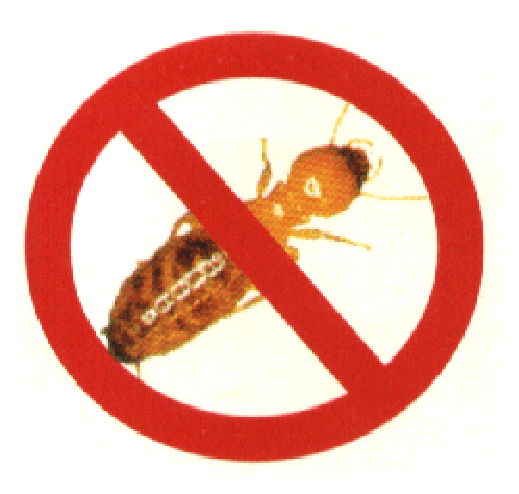
\includegraphics[width=0.5\textwidth]{Cap1/cupim}
%\caption{Proibido estacionar cupins. Legenda grande, com o objetivo de demonstrar a indentação na lista de figuras.}
%\label{cupim}
%\end{figure}

%vê o problema de controle tolerante a falhas através de uma perspectiva integrada, foi proposta por
%{marcel4}. Os autores apresentam um ambiente híbrido consistindo de três unidades básicas que garantem a compleição de tarefas na presença de qualquer número de juntas falhas (Figura \ref{cupim}). A primeira unidade é um esquema de detecção
%e isolação de falhas que continuamente monitora o manipulador para detectar e identificar possíveis falhas nas juntas. A segunda unidade é responsável pela reconfiguração do controle. A terceira unidade é composta de algorítmos de
%controle apropriados para cada tipo de configuração do robô, baseado na informação da unidade de reconfiguração \cite{COFFEE2000}.

%Segundo, o critério de otimização utilizado será o acoplamento entre as juntas do
%manipulador e neste caso, temos um sistema redundante quando ocorre falha de uma das juntas do manipulador de três juntas, e seu posicionamento é controlado pelas duas restantes. Nossa solução para o problema é baseada na formulação
%inversa ({nakamura}). A

%\begin{figure}[ht!]
%\centering
%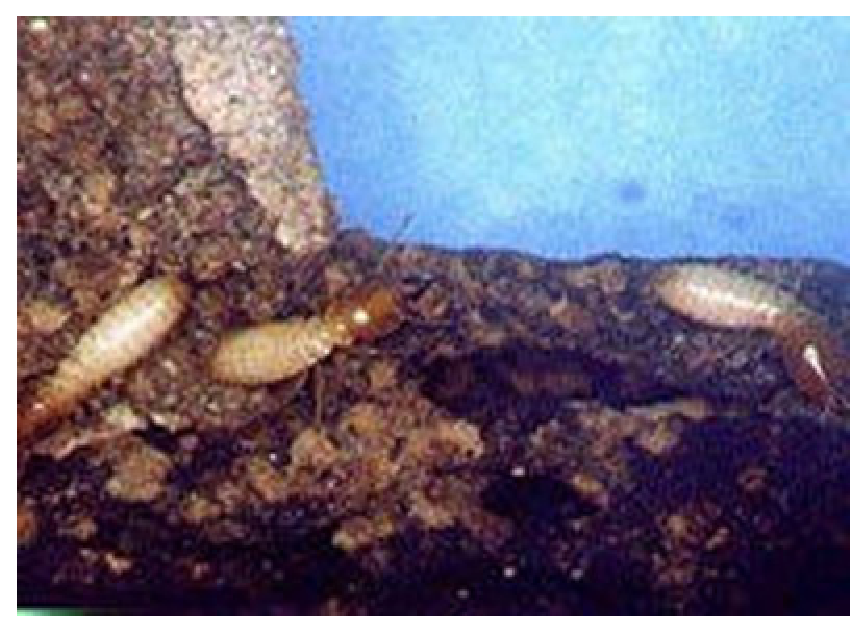
\includegraphics[width=1\textwidth]{Cap1/cupimconcreto}
%\caption{Exemplo real de cupim frente ao seu dilema.}
%\label{FDII}
%\end{figure}


\section{Objective}
	One of the goals of this work is to reune reliable information about the MAVLink protocol in other to become a reference material. In gereral papers related to RPAS applications have a small section about this protocol, but more information is necessary  to undersatand how it works. Although the protocol has its own documentation, many aspects are not explained in details and it lacks a practical use example of the MAVLink inside a simulation environment. 
    
    The second goal is to provide a security analysis of MAVLink protocol using the main strategies commonly used in the literature. Besides the security conclusions, this work aims to show all the details and configurations of the tools used in the study.
%\cite{Nascimento1970}.

%\section{Related Work}

\section{Work Organization}
\subsection{Protocol Overview}
Chapter 2 reports the main aspects of MAVLink in order to contextualize new developers. This chapter aims to follow the MAVLink Developer Guide in order to clarify and complement the official documentation.

\subsection{Simulation Environment}
Chapter \ref{sec_setting_sitl} describe the steps to configure the Software-In-The-Loop enviroment, where the security simulations will take place.

\subsection{Security Analysis of MAVLink}
	This Chapter will start listing the main security issues of the protocol. It also shows different approaches to identify vulnerabilities and how to set up these approaches in a computer.
    
\subsection{New sections}
	New chapters will be included during the work progress. 